\documentclass[12pt]{article}

%% science symbols
\usepackage{amsmath}
\usepackage{amssymb}
\usepackage{amsthm}
\usepackage{bm}
\usepackage{cancel}
\usepackage{physics}
\usepackage{siunitx}
\usepackage{slashed}

%% general pretty stuff
\usepackage{caption}
\usepackage{float}
\usepackage{graphicx}
\usepackage{url}
\usepackage{enumitem}
\usepackage{hyperref}
\usepackage{tikz}
\usepackage{tikz-feynhand}

% setup options
\captionsetup{labelfont=bf}
\graphicspath{ {./figs/} }

% macros
\renewcommand{\L}{\mathcal{L}}
\renewcommand{\H}{\mathcal{H}}
\renewcommand{\l}{\ell}
\newcommand{\M}{\mathcal{M}}
\newcommand{\mcV}{\mathcal{V}}
\newcommand{\D}{\partial}
\newcommand{\veps}{\varepsilon}
\newcommand{\circled}[1]{\tikz[baseline=(char.base)]{
    \node[shape=circle,draw,inner sep=2pt](char){#1};}}

% mdframed environments
\usepackage[framemethod=TikZ]{mdframed}
\mdfsetup{skipabove=\topskip,skipbelow=\topskip}
\mdfdefinestyle{defstyle}{%
  linewidth=1pt,
  frametitlerule=true,
  frametitlebackgroundcolor=gray!40,
  backgroundcolor=gray!20,
  innertopmargin=\topskip
}

\mdtheorem[style=defstyle]{definition}{Definition}
\mdtheorem[style=defstyle]{theorem}{Theorem}
\mdtheorem[style=defstyle]{problem}{Problem}

\newenvironment{thebook}
{\begin{mdframed}[style=defstyle,frametitle={From the Book}]}{\end{mdframed}}

\title{\vspace{-3em}PHYS 167b HW 1}
\author{Michael Cardiff}
\date{January 18, 2024}

\begin{document}
\maketitle

\section{Natural Units}
\begin{problem}
  The following equations are in natural units. Convert them to SI units.
  \begin{enumerate}[label=\alph*)]
  \item $E=\sqrt{p^2+m^2}$
  \item $x^2-t^2=0$
  \item $\pdv{\sigma}{\Omega}=\frac{\alpha^2}{4E^2}(1+\cos^2\theta)$
  \item $m=\frac1{2r_0}$ where $m$ is a mass and $r_0$ is a distance.
  \item The cross section for $e^+e^-\to\mu^+\mu^-$ is $\sigma=\frac{4\pi\alpha^2}{3E_{\text{CM}}^2}$, where $E_{\text{CM}}$ is the center of mass energy. Evaluate the cross section in nanobarns for $E_{\text{CM}}=\SI{10}{\GeV}$. Be careful about the units as the cross section formula is in Natural units
  \end{enumerate}
\end{problem}
\begin{enumerate}[label=\alph*)]
\item I am choosing to keep the energy as an energy here, and adding the required constants to $p$ and $c$ to ``promote'' them to energies, for a $p$ this would be changing it to $pc$ and for a $m$, it would be changing it to $mc^2$, so we end up with:
  \begin{equation}
    \label{eq:p1a}
    \boxed{E=\sqrt{(pc)^2+(mc^2)^2}}
  \end{equation}
\item Here a number of things can be done, but we know in SR, times can be converted to distances via multiplying by $c$, so the replacement $t\to ct$ suffices here:
  \begin{equation}
    \label{eq:p1c}
    \boxed{x^2-c^2t^2=0}
  \end{equation}
\item Here, the quantity on the left is a differential cross section, whose dimensions are $[L^2]$, or an area, the natural units on the left say that it has units of $\unit{GeV^{-2}}$ (since $\alpha$ and things like $\cos\theta$ are dimensionless). In the $[\hbar,c,\unit{\GeV}]$ system, an area is $(\hbar c)^2\unit{\GeV^{-2}}$, so we simply need to multiply by $(\hbar c)^2$ to get the units correct, in order words:
  \begin{equation}
    \label{eq:p2c}
    \boxed{\dv{\sigma}{\Omega}=\frac{\hbar^2c^2\alpha^2}{4E^2}(1+\cos^2\theta)}
  \end{equation}
\item Here to me it is easier to convert both quantites to energies and subsequently simplify. The mass needs to be multiplied by $c^2$, and the distance should be divided by $\hbar c$, the overall effect is:
  \begin{equation}
    \label{eq:p1d}
    mc^2=\frac{\hbar c}{2r_0}\implies
    \boxed{m=\frac{\hbar}{2r_0c}}
  \end{equation}
\item It is worth noting that the conversion for a cross section will be the same as the differential cross section from c, so the overall chain of events will be:
  \begin{align*}
    \sigma^{\text{SI}}=\sigma^{\text{natural}}[\unit{GeV^{-2}}]
    \times(\hbar c)^2[\unit{GeV^2.fm^2}]
    \times\frac{\text{b}}{\SI{100}{fm^2}}
    \times\frac{10^9\text{nb}}{\text{b}}
  \end{align*}
  The cross section in natural units is:
  \begin{align*}
    \sigma^{\text{natual}}=\frac{4\pi\alpha^2}{3E_{\text{CM}}^2}
    =\frac{4\pi\qty(\frac1{137})^2}{3(\SI{10}{GeV})^2}
    \approx\SI{2.2e-6}{GeV^{-2}}
  \end{align*}
  Finally, converting to SI and nb:
  \begin{equation}
    \label{eq:p1e}
    \boxed{\sigma^{\text{SI}}
      =4\pi\frac{\hbar^2c^2\alpha^2}{3E^2_{\text{CM}}}
      \approx0.87\text{ nb}}
  \end{equation}
\end{enumerate}
\newpage
\section{Thomson, Problem 1.5}
\begin{problem}
  Treating the $\pi^0$ as a $u\bar{u}$ bound state, draw the Feynman diagrams for:
  \begin{enumerate}[label=\alph*)]
  \item $\pi^0\to\gamma\gamma$
  \item $\pi^0\to\gamma e^+e^-$
  \item $\pi^0\to e^+e^-e^+e^-$
  \item $\pi^0\to e^+e^-$
  \end{enumerate}
  By considering the number of QED vertices present in each decay, \emph{estimate} the relative decay rates taking $\alpha=1/137$
\end{problem}
\begin{enumerate}[label=\alph*)]
\item The diagram for this process would just be:
  \begin{figure}[H]
    \centering
    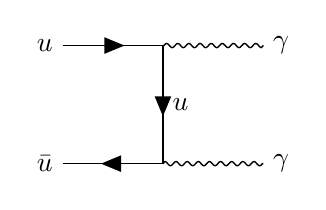
\begin{tikzpicture}
      \begin{feynhand}
        % vertices
        \vertex (p11) at (1.5,0) {$\gamma$};
        \vertex (p21) at (1.5,1.5) {$\gamma$};
        \vertex (p12) at (-1.5,0) {$\bar{u}$};
        \vertex (p22) at (-1.5,1.5) {$u$};
        \vertex (a) at (0,0); \vertex (b) at (0,1.5);
        % particles
        \propag [bos] (p11) to (a);
        \propag [antfer] (p12) to (a);
        \propag [bos] (b) to (p21);
        \propag [fer] (p22) to (b);
        % exchange
        \propag [fer] (b) to [edge label=$u$] (a);
      \end{feynhand}
    \end{tikzpicture}
    \caption{Diagram for problem 2a}
    \label{fig:p2a}
  \end{figure}
  Which has 2 QED vertices, so $\mathcal{M}\propto e^2$ hence $\abs{\mathcal{M}}^2\propto\alpha^2$ and so the decay rate would be proportional to $\alpha^2\approx 1/137^2$.
\item This decay just involves one of the photons decaying into a pair of $e^+e^-$
  \begin{figure}[H]
    \centering
    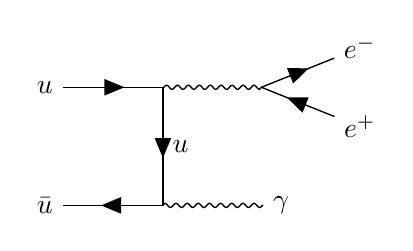
\begin{tikzpicture}
      \begin{feynhand}
        % vertices
        \vertex (p11) at (1.5,0) {$\gamma$};
        \vertex (p21) at (1.25,1.5);
        \vertex (p12) at (-1.5,0) {$\bar{u}$};
        \vertex (p22) at (-1.5,1.5) {$u$};
        \vertex (d1) at (2.5,2.0) {$e^-$};
        \vertex (d2) at (2.5,1.0) {$e^+$};
        \vertex (a) at (0,0); \vertex (b) at (0,1.5);
        % particles
        \propag [bos] (p11) to (a);
        \propag [antfer] (p12) to (a);
        \propag [bos] (b) to (p21);
        \propag [fer] (p22) to (b);
        % exchange
        \propag [fer] (b) to [edge label=$u$] (a);
        % decay
        \propag [fer] (p21) to (d1);
        \propag [antfer] (p21) to (d2);
      \end{feynhand}
    \end{tikzpicture}
    \caption{Diagram for problem 2b}
    \label{fig:p2b}
  \end{figure}
  This process has $3$ QED vertices, so $\M\propto e^3$, $\abs{\M}^2\propto\alpha^3$, so the decay rate is also $\propto\alpha^3$
\item Now both photons decay into pairs!
  \begin{figure}[H]
    \centering
    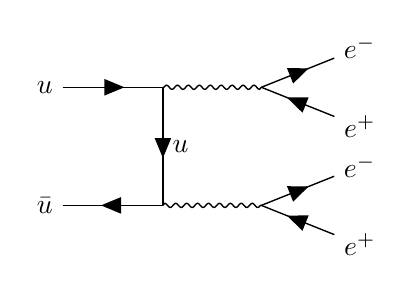
\begin{tikzpicture}
      \begin{feynhand}
        % vertices
        \vertex (p11) at (1.25,0);
        \vertex (p21) at (1.25,1.5);
        \vertex (p12) at (-1.5,0) {$\bar{u}$};
        \vertex (p22) at (-1.5,1.5) {$u$};
        \vertex (d1) at (2.5,2.0) {$e^-$};
        \vertex (d2) at (2.5,1.0) {$e^+$};
        \vertex (d3) at (2.5,0.5) {$e^-$};
        \vertex (d4) at (2.5,-0.5) {$e^+$};
        \vertex (a) at (0,0); \vertex (b) at (0,1.5);
        % particles
        \propag [bos] (p11) to (a);
        \propag [antfer] (p12) to (a);
        \propag [bos] (b) to (p21);
        \propag [fer] (p22) to (b);
        % exchange
        \propag [fer] (b) to [edge label=$u$] (a);
        % decay
        \propag [fer] (p21) to (d1);
        \propag [antfer] (p21) to (d2);
        \propag [fer] (p11) to (d3);
        \propag [antfer] (p11) to (d4);
      \end{feynhand}
    \end{tikzpicture}
    \caption{Diagram for problem 2c}
    \label{fig:p2c}
  \end{figure}
  This diagram has 4 QED vertices, $\M\propto e^4$, $\abs{\M}^2\propto\alpha^4$ and the decay rate is proportional to $\alpha^4$
\item This one has a bit of a different structure, requiring the two quarks annihilate each other:
  \begin{figure}[H]
    \centering
    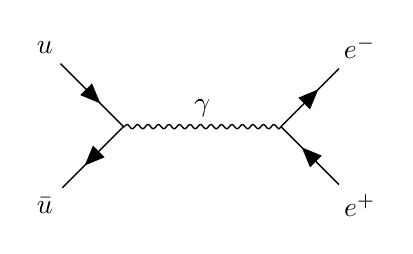
\begin{tikzpicture}
      \begin{feynhand}
        % vertices
        \vertex (p11) at (-1,1) {$u$};
        \vertex (p12) at (-1,-1) {$\bar{u}$};
        \vertex (p21) at (3,1) {$e^-$};
        \vertex (p22) at (3,-1) {$e^+$};
        \vertex (a) at (0,0);
        \vertex (b) at (2,0);
        % particles
        \propag [fer] (p11) to (a);
        \propag [antfer] (p12) to (a);
        \propag [fer] (b) to (p21);
        \propag [antfer] (b) to (p22);
        % loop
        \propag [bos] (a) to [edge label=$\gamma$] (b);
      \end{feynhand}
    \end{tikzpicture}
    \caption{Diagram for problem 2d}
    \label{fig:p2d}
  \end{figure}
  This diagram also has 2 QED verticies, so its $\M$, $\abs{M}^2$ and decay rate should have the same proportionalities as part a.
\end{enumerate}
Seeing as the dominant decay modes are proportional to $\alpha^2$, we should see that decay mode b) should occur about $1/137\approx0.01$ times less than the dominant mode. Decay mode c) then should occur $1/137^2\approx \num{e-4}$ times less than the dominant mode.

\section{Thomson, Problem 1.7}
\begin{problem}
  High-energy muons traversing matter lose energy according to:
  \begin{align*}
    -\frac1\rho\dv{E}{x}\approx a+bE
  \end{align*}
  Where $a$ is due to ionisation energy loss and $b$ is due to the bremsstrahlung and $e^+e^-$ pair-production processes. For standard rock, taken to have $A=22, Z=11,$ and $\rho=\SI{2.65}{g.cm^{-3}}$, the parameters $a$ and $b$ depend only weakly on the muon energy and have values $a\approx\SI{2.5}{MeV.g^{-1}.cm^{2}}$ and $b\approx{3.5e-6}{g^{-1}.cm^{2}}$
  \begin{enumerate}[label=\alph*)]
  \item At what muon energy are the ionisation and bremsstrahlung/pair production processes equally important?
  \item Approximately how far does a $\SI{100}{GeV}$ cosmic-ray muon propagate in rock?
  \end{enumerate}
\end{problem}
\begin{enumerate}[label=\alph*)]
\item The two phenomena should be equally important when $a=bE$, this would give a muon energy of:
  \begin{align*}
    E=\frac{a}{b}
  \end{align*}
  Using the values given:
  \begin{equation}
    \label{eq:p3a}
    \frac{a}{b}\approx\SI{714}{GeV}
  \end{equation}
\item We can get an estimate by separating this equation and integrating both sides:
  \begin{align*}
    -\frac1\rho\dv{E}{x}=a+bE\implies
    \frac{\dd{E}}{a+bE}=-\rho\dd{x}
  \end{align*}
  Integrating from $\SI{100}{GeV}$ to $\SI{0}{GeV}$ in $E$ and $0$ to the propagation length $L$ in $x$:
  \begin{align*}
    \int_{E_0}^0\frac{\dd{E}}{a+bE}&=-\rho\int_0^L\dd{x}\\
    -\frac1b\eval{\log(a+bE)}^0_{E_0}&=\rho\eval{x}_0^L\\
    -\frac1b\eval{\log\frac{a}{a+bE_0}}&=\rho L\\
    \implies\log(1+\frac{b}{a}E_0)&=\rho Lb
  \end{align*}
  Solving for $L$:
  \begin{align*}
    L=\frac1{\rho b}\log(1+\frac{b}{a}E_0)
  \end{align*}
  Plugging in $a,b,E_0,$ and $\rho$ gives:
  \begin{equation}
    \label{eq:p3b}
    \boxed{L\approx\SI{141}{m}}
  \end{equation}
\end{enumerate}

\section{Thomson, Problem 1.8}
\begin{problem}
  Tungsten has a radiation length of $X_0=\SI{0.35}{cm}$ and a critical energy $E_c=\SI{7.97}{MeV}$ . Roughly what thickness of tungsten is required to fully contain a $\SI{500}{GeV}$ electromagnetic shower from an electron?
\end{problem}
Using the equation for $x_{max}$ in the book, we can determine the max number of radiation lengths of tungsten the shower can withstand:
\begin{align*}
  x_{max}=\frac{\log(E/E_c)}{\log(2)}
\end{align*}
Plugging in $E_c=\SI{7.97}{MeV}$ and $E=\SI{500e3}{MeV}$, we get:
\begin{align*}
  x_{max}\approx15.93
\end{align*}
So $\sim15.93$ radiation lengths, multiplying by the rad length given for tungsten:
\begin{equation}
  \label{eq:p4}
  \boxed{x_{max}X_0\approx\SI{5.58}{cm}}
\end{equation}

\section{Thomson, Problem 2.3}
\begin{problem}
  Show that the process $\gamma\to e^+e^-$ can not occur in the vacuum.
\end{problem}
Due to its masslessness, the photon obeys the dispersion relation $E=p$, so its 4 momentum should look like $(E,E\vu{p})$ where $\vu{p}$ is some 3-momentum unit vector. Consider the center of mass frame for the electron positron pair, their 4-momenta would be $(E_{e^+},\vb{p})$ and $(E_{e^-},-\vb{p})$, the total 4-momentum must be conserved, so the photon momentum should be $(E_{e^+}+E_{e^-},\vb{0})$, since the electrons are produced, we know the energy $E_{e^+}+E_{e^-}$ has to be nonzero and at least $2m_e$, but the only possible momentum is $\vb{0}$, so there is no situation where the photon could have produced a pair in the vacuum.

\section{Thomson, Problem 2.9}
\begin{problem}
  Find the maximum opening angle between the photons produced in the decay $\pi^0\to\gamma\gamma$ if the energy of the neutral pion is $\SI{10}{GeV}$, given that $m_{\pi^0}=\SI{135}{MeV}$.
\end{problem}
Assuming the photons scatter into the $y-z$ plane, with $\beta_\pi$ along the $z$ axis. In the $\pi^0$ rest frame, the four-momenta of the photons are:
\begin{align*}
  p_1=(E, 0, E\sin\theta, E\cos\theta)\quad
  p_2=(E, 0,-E\sin\theta,-E\cos\theta)
\end{align*}
Since we are in the rest frame of the $\pi^0$, $E=m_\pi/2$, we then go to the lab frame via the Lorentz transform:
\begin{align*}
  p_x'&=p_x=0\\
  p_y'&=p_y=\pm E\sin\theta\\
  E_1'&=\gamma E_1+\gamma\beta p_{z1}=\gamma E(1+\beta\cos\theta)\\
  E_2'&=\gamma E_2+\gamma\beta p_{z2}=\gamma E(1-\beta\cos\theta)\\
  p_{z1}&=\gamma p_{z1}+\gamma\beta E_1=\gamma E(\beta+\cos\theta)\\
  p_{z2}&=\gamma p_{z2}+\gamma\beta E_2=\gamma E(\beta-\cos\theta)
\end{align*}
We then need to find the angle between the particles in the lab frame, by calculating:
\begin{align*}
  \cos\theta'&=\frac{p'_{x1}p'_{x2}+p'_{y1}p'_{y2}+p'_{z1}p'_{z2}}{E'_1E'_2}\\
  &=\frac{-E^2\sin^2\theta+\gamma^2E^2(\beta^2-\cos^2\theta)}
  {\gamma^2E^2(1-\beta^2\cos^2\theta)}\\
  &=\frac{\beta^2(1+\sin^2\theta)-1}{1-\beta^2\cos^2\theta}
\end{align*}
The extrema of this are $\cos\theta'=-1$ as the minimum, and $\cos\theta'=2\beta^2-1$ as the max. We can go from our parameters to $\beta$ via:
\begin{align*}
  \gamma=\frac{E_\pi}{m_\pi}\approx 74.1 \quad\beta^2=1-\frac1{\gamma^2}
  =1-\frac{m_\pi^2}{E_\pi^2}
\end{align*}
we get the maximum opening angle as:
\begin{equation}
  \label{eq:p6}
  \boxed{\cos(\theta_{min}')=0.973\implies\theta_{min}'=\SI{0.027}{rad}=\ang{1.5}}
\end{equation}
\newpage
\section{Thomson, Problem 2.12}
\begin{problem}
  For the process $1+2\to3+4$, the Mandelstam varuables, $s,t,$ and $u$ are defined as $s=(p_1+p_2)^2$, $t=(p_1-p_3)^2$, and $u=(p_1-p_4)^2$. Show that
  \begin{align*}
    s+u+t=m_1^2+m_2^2+m_3^2+m_4^2
  \end{align*}
\end{problem}
Recalling the fact that for 4-momenta:
\begin{align*}
  p_i^2=m_i^2
\end{align*}
And for any 2 four-vectors:
\begin{align*}
  (a+b)^2=a^2+b^2+2a\vdot b
\end{align*}
It is first useful to expand $s,t,u$ on their own:
\begin{align*}
  s &= (p_1+p_2)^2= p_1^2+p_2^2+2p_1\vdot p_2\\
  t &= (p_1-p_3)^2= p_1^2+p_3^2-2p_1\vdot p_3\\
  u &= (p_1-p_4)^2= p_1^2+p_4^2-2p_1\vdot p_4
\end{align*}
Notice that $s$ and $t$ are both completely written in terms of $p_1,p_2,p_3$, and since 4-momentum is converved, we can rewrite $u$, more importantly $p_4$ as a sum or difference of the other momenta:
\begin{align*}
  p_1+p_2=p_3+p_4\implies p_4=p_1+p_2-p_3
\end{align*}
Hence $u$ can be written as:
\begin{align*}
  u &= (p_1-p_4)^2= p_1^2+p_4-2p_1\vdot(p_1+p_2-p_3)
\end{align*}
Adding the three variables together:
\begin{align*}
  s+t+u &= 3p_1^2+p_2^2+p_3^2+p_4^2+2p_1\vdot(p_2-p_3-p_1-p_2+p_3)\\
  &= 3p_1^2+p_2^2+p_3^2+p_4^2+2p_1\vdot(\cancel{p_2-p_2}-p_1\cancel{-p_3+p_3})\\
  &=(3-2)p_1^2+p_2^2+p_3^2+p_4^2
\end{align*}
Using our initial fact, we get:
\begin{equation}
  \label{eq:p7}
  \boxed{s+t+u=m_1^2+m_2^2+m_3^2+m_4^2}
\end{equation}
\section{Thomson, Problem 1.9}
\begin{problem}
  The CPLEAR detector consisted of: tracking detectors in a magnetic field of $\SI{0.44}{T}$; an electromagnetic calorimeter; and Cherenkov detectors with a radiator of refractive index $n=1.25$ used to distinguish $\pi^\pm$ from $K^\pm$.

  A charged particle travelling perpendicular to the direction of the magnetic field leaves a track with a measured radius of curvature of $R=\SI{4}{m}$. If it is observed to give a Cherenkov signal, is it possible to distinguish between the particle being a pion or kaon? Take $m_\pi\approx\SI{140}{MeV.c^{-2}}$ and $m_K=\SI{494}{MeV.c^{-2}}$.
\end{problem}
From the detector section of the book, we can find the momentum of the particle is (depending on $\lambda$):
\begin{align*}
  p\cos\lambda=0.3 BR=0.3 (0.44) (4)=\SI{0.528}{GeV}=\SI{528}{MeV}
\end{align*}
Note that this the minimum momentum, as the pitch angle would mean dividing by a number less than 1, so this is the lowest possible $p$.

We can only get a Cherenkov signal if the speed of the particle $\beta$ was more than $n^{-1}$ of the detector. This means we need a $\beta>0.8$ for a particle to produce a Cherenkov signal. In terms of the momentum, $\beta=pc/E$ or:
\begin{align*}
  \beta=\frac{p}{\sqrt{(pc)^2+(mc^2)^2}}
\end{align*}
Plugging in $\SI{528}{MeV.c^{-1}}$ for $p$ and both provided values of $m_\pi$ and $m_K$, we find:
\begin{equation}
  \label{eq:p8}
  \begin{aligned}
    \beta_\pi &\approx 0.97\\
    \beta_K &\approx 0.73
  \end{aligned}
\end{equation}
So the particle could \textbf{not} have been a $K^\pm$, but it could have been a $\pi^\pm$
\newpage
\section{Proton Decay}
\begin{problem}
  \begin{enumerate}[label=\alph*)]
  \item Certain beyond the Standard Model (BSM) grand unified theories allow protons to decay. An observation of a proton decay would be a sure sign of New physics. Assuming that we would have noticed if 1\% of the protons in the universe had decayed since the beginning of the Big Bang 13 billion years ago, what limit does this imply for the lifetime of the proton?
  \item The Super-Kamiokande experiment is one of the experiments searching for a proton decay using a 50 kton water tank (Arxiv:2010.16098).
Estimate the 95\% confidence level lower limit on the lifetime of protons assuming no proton decays have been observed so far during the operation of this detector. In Poisson statistics if no events are observed in an experiment the 95\% confidence level lower limit on the number of predicted events is 3 events. Assume that the BSM theories would allow for any of the protons and neutrons in the water molecules to decay with equal lifetime. The molar mass of the water is $\SI{18}{g.mol^{-1}}$.
  \end{enumerate}
\end{problem}
\begin{enumerate}[label=\alph*)]
\item Assuming the exponential decay model we have that:
  \begin{align*}
    N(t)=N(0)e^{-t/\tau}
  \end{align*}
  Where $N(t)$ is the number of protons at time $t$ and $\tau$ is the lifetime. We are given that $N(now)/N(0)\approx0.99$, with $now=\num{1.3e10}$ years, we can then solve for $\tau$ as the only remaining variable:
  \begin{align*}
    0.99=e^{-\num{1.3e10}/\tau}\implies\tau=-\frac{t}{\log(0.99)}
  \end{align*}
  This would give an estimate of:
  \begin{equation}
    \label{eq:p9a}
    \boxed{\tau\approx \num{1.3e12}\text{ year}}
  \end{equation}
\item The 95\% confidence interval is determined by the parameter $\lambda$ which would have produced 3 decays in the operation of the Super-Kamiokande experiment, which is $\sim28$ years. We would then have:
  \begin{align*}
    3=N(0)(1-e^{-t/\tau})
  \end{align*}
  Which is from Poisson statistics. Seeing as the limit from the previous problem was $\order{10^{12}}$ years, it is safe to say that for this experiment $t/\tau\ll1$, so we can rewrite the above as:
  \begin{align*}
    3=N(0)(1-e^{-t/\tau})=N(0)\qty(1-\qty(1-\frac{t}\tau+\order{(t/\tau)^2}))
    \approx N(0)\frac{t}\tau
  \end{align*}
  Hence the lifetime estimate would be:
  \begin{align*}
    \tau=N(0)\frac{28\text{ year}}{3}
  \end{align*}
  All that is left to estimate is $N(0)$, which would be the number of protons and neutrons in the detector when it was turned on 28 years ago. Since we are given a mass of $H_2O$, we can use the molar mass to convert this to mol $H_2O$, convert that to molecules of $H_2O$ using Avogodro's number, and then use the fact that there are 18 nucleons in water:
  \begin{align*}
    N(0)\approx(\SI{50}{\kilo\tonne})
    &\times\qty(\frac{\SI{1e6}{g}}{\SI{1}{\kilo\tonne}})
    \times\qty(\frac{\SI{1}{mol}}{\SI{18}{g}})\\
    &\times\qty(\frac{6.02\times10^{23}\text{ molecule}}{\SI{1}{mol}})
    \times\qty(\frac{18 \text{nucleon}}{1\text{ molecule}})
  \end{align*}
  Plugging in all of these numbers and getting our estimate for $\tau$:
  \begin{equation}
    \label{eq:p9b}
    \boxed{\tau\approx\num{2.8e32}\text{ year}}
  \end{equation}
  Which seems a lot more generous than the previous estimate.
\end{enumerate}
\end{document}